\section{Optical Receiver Device}
\label{TOORD}
The main objective of the \ac{ORD} is to detect the individual energy quanta. A large fraction of the photons emitted by the \acs{laser} are not that easy for detection since they are redirected by the atmosphere, spread due to surface scattering or they are simply absorbed partly by either of them(more detail about atmospheric absorption on appendix ?). The decrease in photon quantity is really severe considering these factors and that is why a photon detector with comparable high quantum efficiency is required. Since the number of photons actually reaching the perimeter of the \ac{ORD} is usually only in the order of one to ten, the \acs{ORD} has to be able to detect and analyze individual small energy packets, preferably single photons. In this section, design option tree is pruned firstly, and there are new approaches after deeply research. After that, trade off is performed which is split up into trade method, trade criteria and weight factor. Finally, trade off summary is drawn.

\subsection{Receiver Prune}
\label{TOReceiverP}
In the design option tree, the GLAS branch is obviously dropped out, since we are trying to improve the whole concept. Meanwhile, the \ac{MPD}'s single-photon detection modules branch has different quantum efficiency for different wavelength. Which means MPD can be a good option for the blue laser detector with 35\% efficiency. The \ac{SPAD} chip could be an approach since it has reasonable high quantum detect efficiency at laser wavelength 450nm. Both \acs{MPD} and \acs{SPAD} are not optimal for \acs{NIR} or \acs{IR} laser detect with low quantum efficiency around 1\%. 

The pruned design option tree for the laser detector can be seen in figure \ref{fig:PrunedReceiver} on page \ref{fig:PrunedReceiver}.

\begin{figure}
\centering
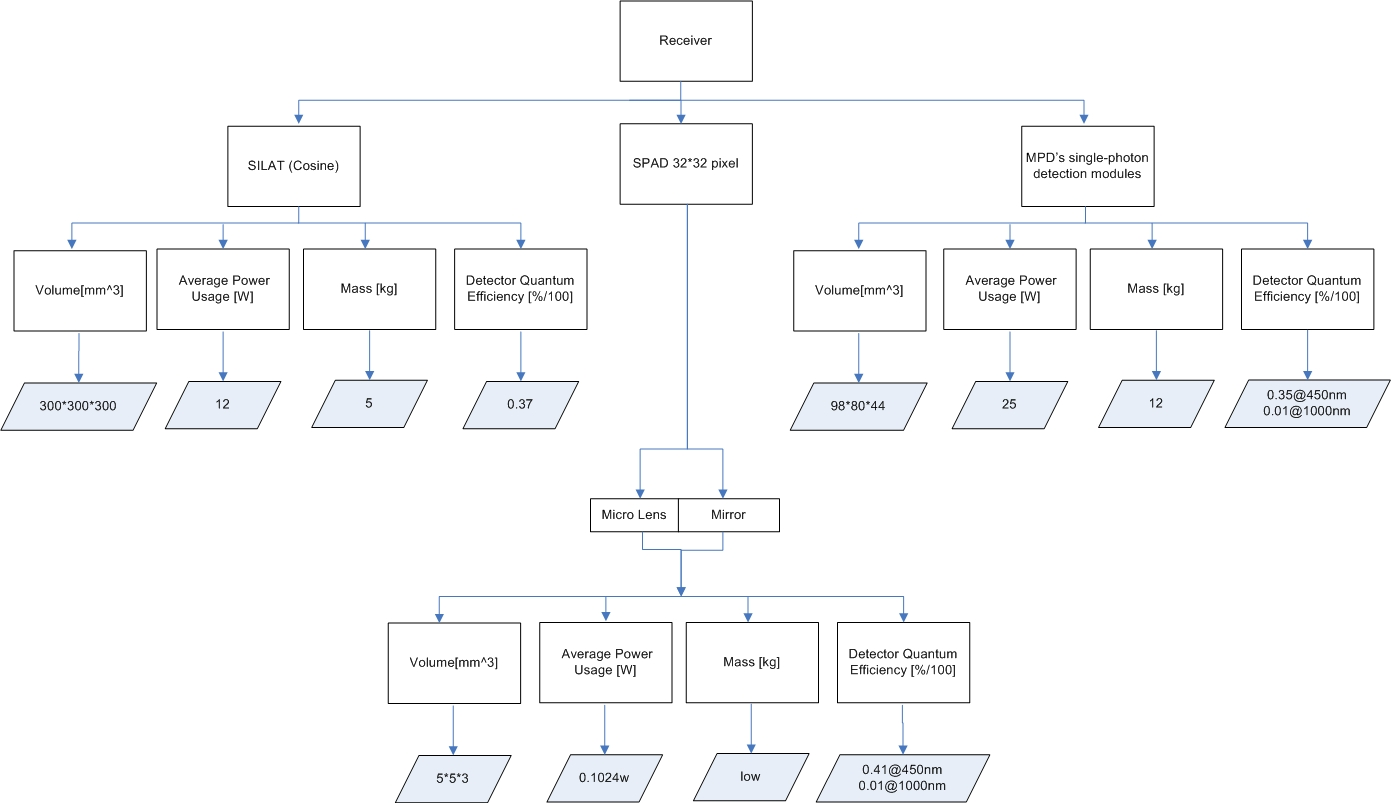
\includegraphics[width=\textheight, angle=90]{chapters/img/DOTreceiverPruned.jpg}
\caption{The pruned design option tree for the Laser receivers}
\label{fig:PrunedReceiver}
\end{figure}

\subsection{Trade Method}
\label{TOReceiverM}
There are mainly four options after pruning and each have different strong points or weak points. 

The first option is \ac{SILAT}, which combines two optical cameras with a low-power photon-counting laser altimeter. It means that \acs{SILAT} operates both pulse laser and photon detector, and it need to be configured as only a photon detector(more information are needed about the configuration). The main strong point is that \acs{SILAT} should has relative higher reliability since it is designed suitable for space mission like spectral imagery and satellite topographic study. 

\ac{MPD}'s photon detection efficiency is obtained through the use of epitaxial silicon \ac{SPAD} and patented \ac{IAQC}, which is specifically designed and optimized for photon counting. The main drawback is that it is difficult to achieve the precise ground resolution due to diffraction.

The final option is use a 32*32 pixel array with in-pixel photon counting, which also use \acs{SPAD} but in \ac{CMOS} technology. It has the highest quantum efficiency for blue laser(@450nm), but only 2\% of the chip area can detect the quanta. In this case, micro lenses or faceted mirrors are used in order to collect most of the incoming quanta focus on such a small area. The solution is shown in figure \ref{fig:diagram_Rgeneral} on page \ref{fig:diagram_Rgeneral}. The parabolic mirror is placed at certain position to the small \acs{SPAD} chip with specified curvature, then the prism barrier is designed to filter other noise lights except wavelength 450nm blue light. After that, different receiver assemblys are designed.
\begin{figure}
\centering
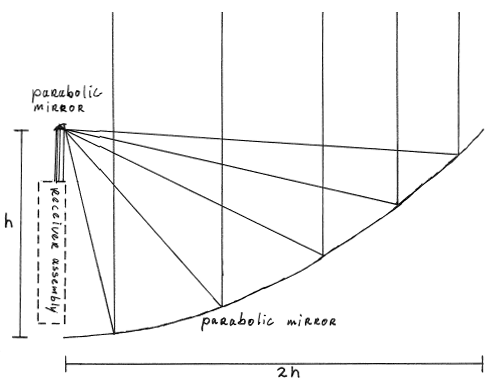
\includegraphics[scale = 0.6]{chapters/img/DiagramReceiverGeneral.png}
\caption{The diagram of the parabolic mirror}
\label{fig:diagram_Rgeneral}
\end{figure}
The draft design diagram of assembly micro lenses is shown on figure \ref{fig:diagram_Rmicrolenses} on page \ref{fig:diagram_Rmicrolenses}. The micro lenses are placed just above the \acs{SPAD} chip to focus light source on the specific pixel 2\% area. On the other hand, the micro lenses could be very heavy due to the high density of the lens material, and it also has high risk of falling off due to vibration during lunching and boosting.
\begin{figure}
\centering
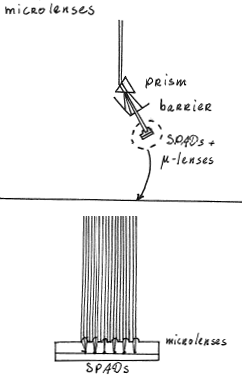
\includegraphics[scale = 0.6]{chapters/img/DiagramReceiverAssemblyMicrolenses.png}
\caption{The diagram receiver assembly micro lenses}
\label{fig:diagram_Rmicrolenses}
\end{figure}
Another way to increase the receiving efficiency is using the faceted mirror such as the figure \ref{fig:diagram_Rfaceted mirror} on page \ref{fig:diagram_Rfaceted mirror} shown. Instead of the heavy micro lenses the multi-faceted elliptical mirror can be placed to achieve the focusing. Since the faceted mirror can reach the same purpose but lighter than micro lenses, it might be a better solution after all. 

\begin{figure}
\centering
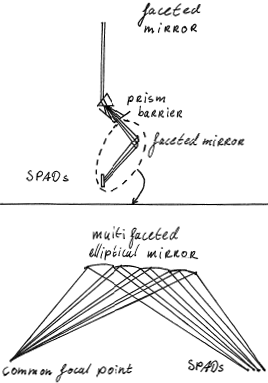
\includegraphics[scale = 0.6]{chapters/img/DiagramReceiverAssemblyFacetedMirror.png}
\caption{The diagram receiver assembly faceted mirror}
\label{fig:diagram_Rfaceted mirror}
\end{figure}


\subsection{Trade Criteria}
\label{TOReceiverC}
In the last paragraph, the general trade off method is elaborated but not in quantity way. It is more precise and clear to give some trade criteria to compare between options, which can be graded from 1-10 (worse to best) to indicate each criterion performance. Mass, power, volume are criteria considered as design of a constellation of micro or nano satellites. The criteria such as efficiency, reliability, resolution and \ac{FOV} are defined whether the receiver can detect photon or not and how precision it could be. Meanwhile, Cost, lifetime and availability need to be noticed generally in each subsystem.

\subsection{Weight Factor}
\label{TOReceiverWF}
Weight factor is given differently to each criterion due to mission objective and instrument performance requirement. Lifetime is the top objective and efficiency determines the photons can be detect or not, so both are given as maximum 10. Power, mass, volume are important since micro or nano receivers are considered. Meanwhile resolution, reliability and \acs{FOV} are also important to perform continuous accurate measurements. The mission objective is about feasibility study, so cost and availability are not the essential part.

\subsection{Trade summary}
\label{TOReceiverS}
The trade off table is shown in figure
\begin{figure}
\centering
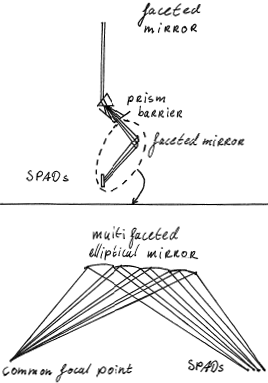
\includegraphics[scale = 0.6]{chapters/img/DiagramReceiverAssemblyFacetedMirror.png}
\caption{The diagram receiver assembly faceted mirror}
\label{fig:diagram_Rfaceted mirror}
\end{figure}
